\documentclass[journal]{IEEEtran}

\usepackage{cite}
\usepackage{amsmath,amssymb}
\usepackage{graphicx}
\usepackage{booktabs}
\usepackage{multirow}
\usepackage{array}
\usepackage[table]{xcolor}
\usepackage{url}
\usepackage[hidelinks]{hyperref}

\newcommand{\best}[1]{\textbf{#1}}
\newcommand{\fcha}{FCHA}
\renewcommand{\arraystretch}{1.12}

\begin{document}

\title{Flow-Conditioned Host Attention for Federated Intrusion Detection in IoT Networks: A Leakage-Controlled Evaluation on Unseen Traffic and Unseen Attackers}

\author{Author~One,~\IEEEmembership{Member,~IEEE,}
        Author~Two,
        Author~Three,
        and~Author~Four%
\thanks{The authors are with [Department], [Institution], [City, Country] (e-mail: [address]).}%
\thanks{Code, configuration files and all per-run results are available at [repository URL].}}

\markboth{IEEE Transactions on [Journal Name],~Vol.~XX, No.~X, Month~2026}%
{Author One \MakeLowercase{\textit{et al.}}: Flow-Conditioned Host Attention for Federated IoT Intrusion Detection}

\maketitle

\begin{abstract}
Graph neural networks (GNNs) for network intrusion detection usually summarise each host by averaging the flows it sends and receives. When one host mixes benign traffic with several attack types, as is common in IoT testbeds, this average is dominated by the majority traffic and the minority attack becomes invisible. We propose Flow-Conditioned Host Attention (FCHA), an edge classifier in which the flow being classified is the attention query over the other flows of its sender and of its receiver, so the context of each flow is assembled mainly from traffic that resembles it. FCHA is trained fully federatedly: model weights, feature standardisation statistics and model-selection signals are all aggregated across clients, and no raw flow, label or host identity leaves a client. We evaluate it under a leakage-controlled protocol that caps duplicated flows, splits data by flow signature (unseen traffic patterns) and by attacker host (unseen attackers), repeats every configuration over 5 folds and 3 seeds, and tests differences with Holm-corrected paired Wilcoxon tests. On three benchmarks (NF-ToN-IoT-v2, ToN-IoT-Network, NF-CSE-CIC-IDS2018-v2), FCHA is the best federated model on unseen traffic patterns, reaching 94.2\%, 99.1\% and 95.6\% balanced accuracy against 91.4\%, 98.6\% and 83.9\% for centralised XGBoost ($p<0.001$), and raising recall of rare classes such as web attacks from at most 31.4\% to 80.4\%. Host-level averaging, the aggregation used by recent federated GNN detectors, loses up to 22 points. On unseen attackers every model degrades sharply; FCHA has the best mean on two of three datasets with the lowest false-positive rate of all models (6.0\% and 4.9\%, against 16.5--22.1\% and 6.3--10.8\% for the tree ensembles), whereas a centralised random forest is best on the third. Federated FCHA matches its centralised counterpart under IID clients. We release the full protocol so that results on these benchmarks can be compared on equal terms.
\end{abstract}

\begin{IEEEkeywords}
Intrusion detection, Internet of Things, federated learning, graph neural networks, attention, NetFlow, data leakage, evaluation methodology.
\end{IEEEkeywords}

\section{Introduction}
\IEEEPARstart{I}{nternet} of Things (IoT) deployments connect large numbers of heterogeneous, weakly protected devices, and network intrusion detection systems (NIDS) remain a primary line of defence for them. Training a learned NIDS needs labelled traffic from many sites, yet operators are rarely willing or allowed to pool raw flow records, which reveal internal addressing, services and user behaviour. Federated learning (FL)~\cite{mcmahan2017fedavg,li2020flchallenges} addresses this by training a shared model while each site keeps its traffic local.

Network traffic is naturally a graph: hosts are nodes and flows are directed edges between them. GNN-based NIDS exploit this structure by enriching each flow with information about its endpoints. E-GraphSAGE~\cite{lo2022egraphsage} aggregates the features of the flows incident to each host and classifies a flow from its own features together with its two endpoint embeddings, and later work added residual connections and attention between hosts~\cite{chang2024eresgat}. Federated variants extend this idea across organisations; FedGATSage~\cite{altfaily2025fedgatsage}, for example, combines client-side graph attention with a server-side GraphSAGE overlay~\cite{hamilton2017graphsage} and reports results comparable to centralised training.

These architectures share a design choice that we argue is harmful for IoT traffic: a host is represented by an aggregate over \emph{all} of its flows. In the ToN-IoT testbed, for instance, a small number of attacker machines each emit several attack types alongside benign traffic. When such a host is summarised by an average, the summary is dominated by its most frequent traffic, and a flow from a rarer attack receives a context that resembles a different class. Mean aggregation therefore helps majority classes and can actively hurt minority ones, which are exactly the attacks a NIDS most needs to detect.

A second difficulty is evaluation. Public NIDS benchmarks contain massive exact duplication: keeping at most ten copies of each identical record reduces the 16{,}809 Backdoor flows of NF-ToN-IoT-v2 to 239, and the 143{,}097 Bot flows of NF-CSE-CIC-IDS2018-v2 to 997. Random flow-level splits place copies of the same record in training and test sets, and the test then measures memorisation. Pitfalls of this kind, including data snooping and inappropriate baselines, are widespread in security applications of machine learning~\cite{arp2022dos}. Many published federated GNN detectors do not state how their test sets were drawn, which makes their numbers difficult to interpret or compare.

This paper addresses both issues. Our contributions are:
\begin{enumerate}
\item \textbf{FCHA, a flow-conditioned aggregator.} The flow being classified acts as the attention query over the flows of its sender and of its receiver, so each flow builds its own context from similar traffic rather than from a host-wide average (Section~\ref{sec:method}). Baselines with mean aggregation, host-only aggregation and no graph share the same code path, so differences isolate the aggregator.
\item \textbf{A fully federated pipeline.} Feature standardisation is computed from aggregated client moments, model selection from aggregated client validation confusion counts, and weights with FedAvg. Raw flows, per-flow labels and host addresses never leave a client.
\item \textbf{A leakage-controlled protocol.} We cap exact duplicates, use a signature-grouped split for unseen traffic patterns and a leave-attacker-out split for unseen attackers, guard against label leakage automatically, include a shuffled-label sanity check, and report 5 folds $\times$ 3 seeds with Holm-corrected paired tests (Section~\ref{sec:protocol}).
\item \textbf{An extensive, honest comparison} on three benchmarks against graph baselines, a federated flow-only network and centralised tree ensembles, including an analysis of when host context helps and when it does not (Sections~\ref{sec:results}--\ref{sec:discussion}).
\end{enumerate}

Our results show that, when attackers are seen during training, FCHA clearly outperforms flow-only models and tree ensembles and matches or exceeds mean aggregation, with the largest gains on rare classes; on unseen attackers the gap closes, where a well-tuned tree ensemble remains a strong reference but raises substantially more false alarms on two of the three datasets.

\section{Related Work}
\label{sec:related}

\subsection{Graph Neural Networks for Intrusion Detection}
GNNs learn node or edge representations by aggregating information from graph neighbourhoods. GraphSAGE~\cite{hamilton2017graphsage} introduced inductive neighbourhood sampling and aggregation, and graph attention networks (GAT)~\cite{velickovic2018gat} weight neighbours by learned attention coefficients. In NIDS, flows are edges carrying the informative features, so node-centric models must be adapted. E-GraphSAGE~\cite{lo2022egraphsage} aggregates incident edge features into host embeddings and concatenates the embeddings of both endpoints to classify an edge. Chang and Branco~\cite{chang2024eresgat} added residual connections to E-GraphSAGE and proposed E-ResGAT, an attention-based variant. Ngo~\emph{et al.}~\cite{ngo2025attribute} study attribute-based graph construction for IoT intrusion detection. Temporal graph networks~\cite{rossi2020tgn} model dynamic interaction graphs and are a natural extension for streaming traffic. In these models attention, where present, is computed between hosts or between a host and its neighbours; the flow under classification does not decide which of its endpoint's flows are relevant. FCHA makes exactly this decision.

\subsection{Federated Intrusion Detection}
FL trains a global model by repeatedly averaging locally updated weights~\cite{mcmahan2017fedavg}. Statistical heterogeneity across clients is its central difficulty~\cite{li2020flchallenges}: label-skewed partitions degrade FedAvg considerably~\cite{zhao2018noniid}, and Dirichlet label sampling is the standard way to simulate such skew~\cite{hsu2019noniid}. Federated GNNs raise additional questions about where graph structure lives and which statistics are shared~\cite{liu2024fedgnn}. For intrusion detection, FedGATSage~\cite{altfaily2025fedgatsage} aggregates groups of nodes into communities on each client before sending them to a GraphSAGE model on the server, reporting 78.58\% balanced accuracy on NF-ToN-IoT. FedSTGCN~\cite{wang2025fedstgcn} combines spatial and temporal graph convolutions in a federated setting, and Youm and Kim~\cite{youm2025sampling} address class imbalance in federated detection with class-specific dynamic sampling. These systems are typically evaluated on random splits whose treatment of duplicates and of attacker identity is not reported, and most share a host-level aggregation step. Our work is complementary: we change the aggregation and evaluate it under a protocol designed to expose leakage.

\subsection{Datasets and Evaluation Pitfalls}
The NetFlow-based benchmarks of Sarhan~\emph{et al.}~\cite{sarhan2021netflow,sarhan2022standard} convert several public datasets, including ToN-IoT~\cite{moustafa2021toniot,alsaedi2020toniot} and CSE-CIC-IDS2018~\cite{sharafaldin2018cicids}, to a common NetFlow feature set, which allows models to be compared across networks. Arp~\emph{et al.}~\cite{arp2022dos} identify recurring pitfalls in security machine learning, among them sampling bias, data snooping through information shared between training and test sets, and weak baselines. Two of these are acute for flow benchmarks: duplicated records spanning the train/test boundary, and attacker hosts present in both. We address the first with duplicate capping and signature-grouped splits, and the second with a leave-attacker-out split. We also always include strong centralised tree ensembles~\cite{breiman2001rf,chen2016xgboost}, which on flow features are frequently competitive with deep models.

\section{Problem Formulation}
\label{sec:problem}
Each client $k\in\{1,\dots,K\}$ observes a set of flows $\mathcal{E}_k$. A flow $e=(u,v,\mathbf{x}_e,y_e)$ goes from source host $u$ to destination host $v$, has a feature vector $\mathbf{x}_e\in\mathbb{R}^d$ (NetFlow or Zeek fields after encoding) and a class label $y_e\in\{1,\dots,C\}$ (benign or one of several attack types). The flows of a client induce a directed multigraph $G_k=(V_k,\mathcal{E}_k)$ whose nodes are hosts. The task is multi-class flow classification. Host addresses define the graph but are never used as features.

\emph{Federation and privacy model.} Clients do not share flows, labels or host addresses. They may share model parameters, aggregate feature moments (count, sum and sum of squares per feature) and aggregate validation confusion counts. We assume an honest-but-curious server and do not add formal privacy mechanisms such as differential privacy; their combination with FCHA is left to future work (Section~\ref{sec:discussion}).

\emph{Inference.} At test time a deployed model observes a window of unlabelled traffic. We build the test graph from test flows only, so the context of a test flow consists of other test flows; no training flow or label is visible during inference.

\section{Flow-Conditioned Host Attention}
\label{sec:method}

\begin{figure*}[t]
\centering
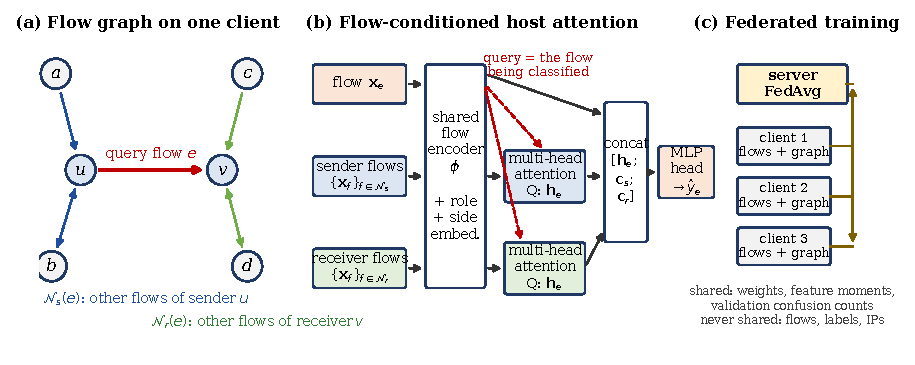
\includegraphics[width=\textwidth]{figures/fig_arch.pdf}
\caption{Overview. (a) A query flow $e$ from $u$ to $v$ and the other flows incident to its endpoints. (b) FCHA encodes all flows with a shared encoder, then attends separately over the sender's and the receiver's flows, using the query flow as the attention query; the two contexts and the flow's own embedding are concatenated and classified. (c) Training is federated: only weights, feature moments and validation confusion counts are exchanged.}
\label{fig:arch}
\end{figure*}

Fig.~\ref{fig:arch} gives an overview. All neural models in this paper share the encoder, classification head, loss and training procedure, and differ only in how endpoint context is aggregated.

\subsection{Flow Encoder and Neighbourhoods}
A shared encoder $\phi$ maps flow features to a $D$-dimensional embedding, $\mathbf{h}_e=\phi(\mathbf{x}_e)$, where $\phi$ is a two-layer perceptron with layer normalisation and GELU activation. For a query flow $e=(u,v)$ we define its sender neighbourhood $\mathcal{N}_s(e)$ as the other flows incident to $u$ and its receiver neighbourhood $\mathcal{N}_r(e)$ as the other flows incident to $v$, in either direction. To bound cost on high-degree hosts, each neighbourhood is enumerated exactly when the host has at most $M$ incident flows and otherwise sampled uniformly with replacement to $M$ flows; the query flow itself is always excluded. Each neighbour embedding is tagged with the role the host plays in that neighbour flow (sender or receiver) and with the side of the query it belongs to:
\begin{equation}
\tilde{\mathbf{h}}_f^{(t)} = \phi(\mathbf{x}_f) + \boldsymbol{\rho}_{\mathrm{role}(f)} + \boldsymbol{\sigma}_t,\qquad f\in\mathcal{N}_t(e),\; t\in\{s,r\},
\end{equation}
where $\boldsymbol{\rho}$ and $\boldsymbol{\sigma}$ are learned embeddings.

\subsection{Flow-Conditioned Attention}
For each side $t$ and each of $H$ heads, the query is computed from the flow being classified and the keys and values from its neighbours:
\begin{align}
\mathbf{q}^{(t)} &= \mathbf{W}_Q(\mathbf{h}_e+\boldsymbol{\sigma}_t),\quad
\mathbf{k}_f^{(t)} = \mathbf{W}_K\tilde{\mathbf{h}}_f^{(t)},\quad
\mathbf{v}_f^{(t)} = \mathbf{W}_V\tilde{\mathbf{h}}_f^{(t)},\\
\alpha_{ef}^{(t)} &= \frac{\exp\!\big(\mathbf{q}^{(t)\top}\mathbf{k}_f^{(t)}/\sqrt{D/H}\big)}{\sum_{g\in\mathcal{N}_t(e)}\exp\!\big(\mathbf{q}^{(t)\top}\mathbf{k}_g^{(t)}/\sqrt{D/H}\big)},\\
\mathbf{c}_t &= \mathbf{W}_O\,\big\Vert_{h=1}^{H}\sum_{f\in\mathcal{N}_t(e)}\alpha_{ef}^{(t,h)}\mathbf{v}_f^{(t,h)},
\end{align}
using scaled dot-product attention~\cite{vaswani2017attention} with per-head projections (head index omitted in the first two lines). A host with no other flow contributes a zero context. The flow is classified from its own embedding and its two contexts,
\begin{equation}
\hat{\mathbf{p}}_e=\mathrm{softmax}\big(\mathbf{W}_c\,\psi([\mathbf{h}_e;\mathbf{c}_s;\mathbf{c}_r])\big),
\end{equation}
where $\psi$ is a two-layer perceptron. Because $\alpha_{ef}$ depends on the query flow, two flows on the same host can draw entirely different contexts from it: on a host that sends both benign traffic and a rare attack, a flow of the rare attack can place most of its attention on similar flows. This is the property mean aggregation lacks.

\subsection{Baselines in the Same Code Path}
Replacing the attention weights by uniform weights $\alpha_{ef}=1/|\mathcal{N}_t(e)|$ gives \emph{E-GraphSAGE-mean}, an edge classifier in the style of~\cite{lo2022egraphsage} with mean context and the flow's own features. Dropping $\mathbf{h}_e$ from the classifier input as well gives \emph{Host-mean}, which classifies a flow only from averages over its endpoints, the aggregation underlying host-level federated GNN detectors such as~\cite{altfaily2025fedgatsage}. Removing both contexts gives \emph{Flow-MLP}, a flow-only network. All four models are trained with the same loss, optimiser and federated procedure.

\subsection{Loss}
We use class-weighted cross-entropy. Each client computes weights from its \emph{local} class counts $n_c$ as $w_c\propto n_c^{-1/2}$, normalised to mean one over the classes it holds; inverse-square-root weights are a mild correction that avoids the instability of full inverse-frequency weighting on very rare classes~\cite{johnson2019imbalance,cui2019classbalanced}. As an ablation we add a supervised contrastive term~\cite{khosla2020supcon} on the penultimate representation (weight 0.1, temperature 0.1).

\subsection{Fully Federated Training}
\label{sec:fed}
Training follows FedAvg~\cite{mcmahan2017fedavg} with three additions that keep every stage federated.

\emph{Standardisation.} Each client sends the count, sum and sum of squares of every feature over its training flows. The server combines them into global means and standard deviations, which all clients and the test pipeline use. This is identical to standardising the pooled data but needs no raw values.

\emph{Model selection.} Each client holds out 10\% of its flows for validation, grouped by flow signature so that duplicates do not cross the boundary. After every round, clients evaluate the global model on their validation flows and send the confusion matrix; the server sums the matrices, computes balanced accuracy and keeps the best round. Training stops after 10 rounds without improvement.

\emph{Weights.} Each round every client trains for one local epoch (at most 600 steps of batch size 512, AdamW, learning rate $3\times10^{-4}$, weight decay $10^{-4}$, gradient clipping at 5) and the server averages the weights in proportion to local training sizes, for at most 30 rounds.

\subsection{Complexity and Communication}
With neighbourhood size $M$, the cost of classifying one flow is $O(M D)$ regardless of host degree, so FCHA scales linearly in the number of flows. With $D=128$, $H=4$ and $M=16$, FCHA has 171k parameters (0.68\,MB in 32-bit floats), compared with 121k for E-GraphSAGE-mean, 105k for Host-mean and 72k for Flow-MLP. Per round each client downloads and uploads one copy of the weights.

\section{Experimental Protocol}
\label{sec:protocol}

\subsection{Datasets}
Table~\ref{tab:datasets} summarises the three benchmarks. NF-ToN-IoT-v2 and NF-CSE-CIC-IDS2018-v2 are the NetFlow versions~\cite{sarhan2022standard} of ToN-IoT~\cite{moustafa2021toniot} and CSE-CIC-IDS2018~\cite{sharafaldin2018cicids}; ToN-IoT-Network is the original ToN-IoT network training/testing set with Zeek connection, DNS, HTTP and SSL fields. For the two large NetFlow sets we read at most 150{,}000 flows per class in a single pass (all flows of rarer classes are kept). As in~\cite{altfaily2025fedgatsage}, the Ransomware and MITM classes of ToN-IoT are dropped. The 15 raw CSE-CIC-IDS2018 labels are merged into 7 families.
NF-ToN-IoT-v2 and ToN-IoT-Network come from the same testbed and share attacker machines; NF-CSE-CIC-IDS2018-v2 is an independent network.

\begin{table}[t]
\centering
\caption{Datasets after duplicate capping (at most 10 copies of each identical flow).}
\label{tab:datasets}
\setlength{\tabcolsep}{4pt}
\footnotesize
\begin{tabular}{@{}lrrcc@{}}
\toprule
Dataset & Flows read & After cap & Classes & Features \\
\midrule
NF-ToN-IoT-v2 & 1{,}066{,}809 & 396{,}551 & 8 & 158 \\
ToN-IoT-Network & 190{,}000 & 130{,}248 & 8 & 153 \\
NF-CSE-CIC-IDS2018-v2 & 833{,}872 & 280{,}632 & 7 & 148 \\
\bottomrule
\end{tabular}
\end{table}

\subsection{Features and Leakage Guards}
Numeric fields are transformed with $\mathrm{sign}(x)\log(1+|x|)$; we add derived features (byte and packet asymmetry, bytes per packet, byte rate), bucket ports into well-known, registered and ephemeral ranges, and one-hot encode categorical fields with vocabularies learned from training data only. Labels, the binary attack flag, flow identifiers and IP addresses are never features. An automatic scan rejects any column whose value determines the label on the training data. Such a column is easy to introduce by accident: a label-index column left among the features made an earlier version of our pipeline score 93\% balanced accuracy on random-noise data.

\subsection{Duplicate Capping}
Exact duplicates are frequent: capping keeps only 37\% of the NF-ToN-IoT-v2 flows and 34\% of the NF-CSE-CIC-IDS2018-v2 flows, and individual classes are far more repetitive (Backdoor: 16{,}809 flows reduced to 239; Bot: 143{,}097 reduced to 997). We keep at most 10 copies of each identical flow before splitting. Without the cap, signature-grouped folds were badly unbalanced (one NF-CSE-CIC-IDS2018-v2 test fold consisted of 66\% Bot flows and contained 9 brute-force flows).

\subsection{Splits}
\emph{Signature split (unseen flow patterns).} A flow's signature is the tuple (destination port, protocol, inbound and outbound bytes and packets, duration). We apply 5-fold StratifiedGroupKFold with signatures as groups, so no test flow has an identical copy in training. Every fold has zero signature overlap.

\emph{Leave-attacker-out split (unseen attackers).} We identify attacker hosts as sources of at least 50 attack flows and distribute them over 5 folds, heaviest first, each assigned to the fold with the fewest attack flows so far; all other source hosts are assigned at random. A test fold contains every flow sent by its hosts, and no flow sent by a test host appears in training. Table~\ref{tab:attackerfolds} lists the held-out attackers of ToN-IoT-Network. Because a class whose only attacker is held out cannot be learned, we report balanced accuracy over \emph{supported} classes (at least 50 test flows and present in training).

A plain $K$-fold over all source hosts is unsuitable for these benchmarks: each attack class is generated by only a handful of attacker machines among hundreds of hosts, so most folds hold no attack at all (in our trial on NF-ToN-IoT-v2, three of five test folds had 4--865 flows and no attack).

\begin{table}[t]
\centering
\caption{Leave-attacker-out folds on ToN-IoT-Network: held-out attacker and attack classes tested (training flows of the same class from other machines in brackets).}
\label{tab:attackerfolds}
\setlength{\tabcolsep}{3pt}
\footnotesize
\begin{tabular}{@{}cl p{5.0cm}@{}}
\toprule
Fold & Attacker & Attack classes tested \\
\midrule
F0 & .1.30 & DDoS 14{,}215 (2{,}647), DoS 18{,}578 (1{,}296), injection 7{,}813 (12{,}081), password 8{,}609 (9{,}124), scanning 5{,}910 (6{,}862)\\
F1 & .1.31 & DDoS 2{,}643 (14{,}219), DoS 603 (19{,}271), injection 12{,}080 (7{,}814), password 9{,}124 (8{,}609), scanning 1{,}974 (10{,}798)\\
F2 & .1.32 & scanning 4{,}888 (7{,}884), XSS 8{,}275 (537)\\
F3 & .1.193 & Backdoor 6{,}817 (143)\\
F4 & 4 minor & Backdoor 143, DoS 692, XSS 537\\
\bottomrule
\end{tabular}
\end{table}

\subsection{Clients}
Training data are partitioned over $K=5$ clients either IID or with Dirichlet label skew ($\alpha=0.5$, at least 200 flows per client)~\cite{hsu2019noniid}. FCHA and Flow-MLP are run under both; the graph baselines under IID. Each client builds its graph only from its own flows.

\subsection{Models and Baselines}
Besides FCHA ($D=128$, $H=4$, $M=16$, dropout 0.1) and the three same-code-path baselines, we train a random forest (200 trees)~\cite{breiman2001rf} and XGBoost (300 trees, depth 8, learning rate 0.1)~\cite{chen2016xgboost} on the same features. The tree models are trained \emph{centrally} on pooled data, an advantage the federated models do not have; they are marked $\dagger$. Two ablations are run on the signature split: FCHA with the supervised contrastive term, and centralised FCHA (one client).

\subsection{Metrics and Statistics}
The primary metric is balanced accuracy (mean per-class recall), robust to the strong class imbalance; we also report macro-F1 and the false-positive rate (fraction of benign flows flagged as attacks). Every configuration is run on all 5 folds with seeds 42, 43 and 44, i.e.\ 15 runs, and we report the mean $\pm$ sample standard deviation. Differences to FCHA are tested with the two-sided paired Wilcoxon signed-rank test~\cite{wilcoxon1945} over the 15 matched (fold, seed) pairs, with Holm's correction~\cite{holm1979} within each table. As a sanity check, FCHA is also trained once per fold on randomly permuted labels; it must score at chance.

\subsection{Implementation}
The pipeline is implemented in PyTorch and scikit-learn. Graph models ran mostly on NVIDIA T4 GPUs and partly on CPU; all runs of a configuration share the same code and configuration files, and a run's identity is a hash of every setting that affects its result, so runs from different machines can be merged without duplication.

\section{Results}
\label{sec:results}

\begin{figure*}[t]
\centering
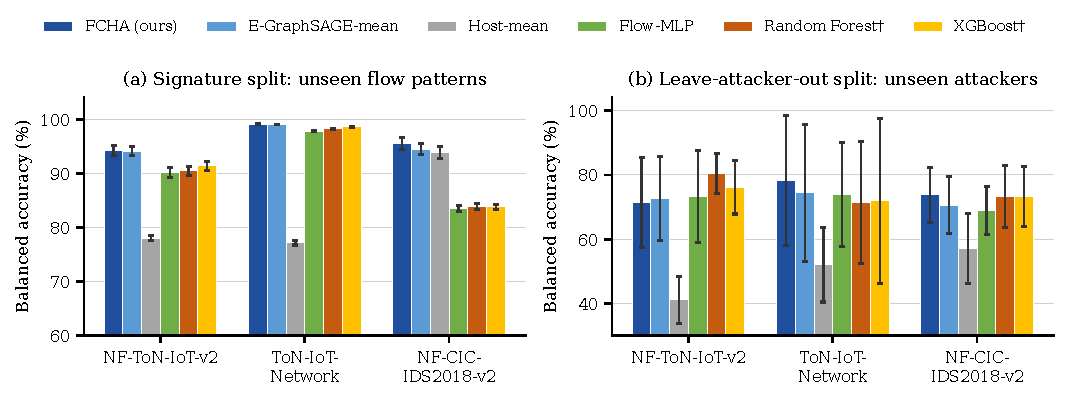
\includegraphics[width=\textwidth]{figures/fig_main.pdf}
\caption{Balanced accuracy (mean $\pm$ SD over 5 folds $\times$ 3 seeds, IID clients) on (a) the signature split and (b) the leave-attacker-out split. $\dagger$: centralised.}
\label{fig:main}
\end{figure*}

\subsection{Unseen Flow Patterns}
Table~\ref{tab:signature} and Fig.~\ref{fig:main}(a) report the signature split. FCHA has the highest balanced accuracy on all three datasets (tied with E-GraphSAGE-mean on ToN-IoT-Network) and is significantly better than every flow-only model and both tree ensembles ($p<0.001$). The largest gain is on NF-CSE-CIC-IDS2018-v2, where FCHA reaches 95.6\% balanced accuracy against 83.9\% for both centralised tree models and 83.5\% for Flow-MLP. ToN-IoT-Network is close to saturated: every model except Host-mean exceeds 97.7\%, and FCHA's lead over XGBoost is 0.5 points.

Mean aggregation of endpoint context (E-GraphSAGE-mean) is close to FCHA on NF-ToN-IoT-v2 (94.1 vs 94.2, not significant) and on ToN-IoT-Network, and 1.1 points behind on NF-CSE-CIC-IDS2018-v2 ($p<0.001$). Host-mean, which drops the flow's own features, loses 16.2 and 21.9 points on the two ToN-IoT datasets and flags 31.0\% of benign flows as attacks on NF-ToN-IoT-v2. On NF-CSE-CIC-IDS2018-v2 it is only 1.7 points behind FCHA. This contrast is informative: in CSE-CIC-IDS2018 most attacker machines run a single attack type, so a host average identifies the attack, whereas in ToN-IoT the attackers mix several attack types with benign traffic, and the average hides them.

For reference, FedGATSage reports 78.58\% balanced accuracy on NF-ToN-IoT~\cite{altfaily2025fedgatsage}; our Host-mean baseline, which uses the same kind of host-level aggregation, reaches 78.0\% on NF-ToN-IoT-v2 under our protocol, and FCHA reaches 94.2\%. The dataset version and split differ, so this is indicative rather than a like-for-like comparison.

\begin{table}[t]
\centering
\caption{Signature split (unseen flow patterns), IID clients. Mean $\pm$ SD over 15 runs. BA: balanced accuracy, F1: macro-F1, FPR: false-positive rate (\%). $p$: Holm-corrected Wilcoxon test vs.\ FCHA. $\dagger$: centralised.}
\label{tab:signature}
\setlength{\tabcolsep}{2.6pt}
\footnotesize
\begin{tabular}{@{}lcccc@{}}
\toprule
Model & BA & F1 & FPR & $p$ \\
\midrule
\multicolumn{5}{@{}l}{\emph{NF-ToN-IoT-v2}}\\
FCHA (ours) & \best{94.2}$\pm$0.9 & \best{92.2}$\pm$1.5 & 4.6$\pm$0.3 & -- \\
E-GraphSAGE-mean & 94.1$\pm$0.9 & 92.0$\pm$1.7 & 4.5$\pm$0.4 & 0.095 \\
Host-mean & 78.0$\pm$0.5 & 74.9$\pm$1.5 & 31.0$\pm$1.0 & $<$0.001 \\
Flow-MLP & 90.1$\pm$0.9 & 87.2$\pm$2.2 & 6.7$\pm$0.8 & $<$0.001 \\
Random Forest$\dagger$ & 90.5$\pm$0.8 & 91.1$\pm$0.8 & \best{3.5}$\pm$0.3 & $<$0.001 \\
XGBoost$\dagger$ & 91.4$\pm$0.9 & 91.7$\pm$0.8 & 4.8$\pm$0.4 & $<$0.001 \\
\midrule
\multicolumn{5}{@{}l}{\emph{ToN-IoT-Network}}\\
FCHA (ours) & \best{99.1}$\pm$0.1 & \best{99.1}$\pm$0.1 & \best{0.1}$\pm$0.1 & -- \\
E-GraphSAGE-mean & \best{99.1}$\pm$0.1 & 99.0$\pm$0.1 & \best{0.1}$\pm$0.1 & 0.008 \\
Host-mean & 77.2$\pm$0.4 & 76.9$\pm$0.4 & 0.2$\pm$0.1 & $<$0.001 \\
Flow-MLP & 97.8$\pm$0.1 & 97.4$\pm$0.1 & 0.7$\pm$0.1 & $<$0.001 \\
Random Forest$\dagger$ & 98.3$\pm$0.1 & 98.3$\pm$0.1 & 0.3$\pm$0.1 & $<$0.001 \\
XGBoost$\dagger$ & 98.6$\pm$0.1 & 98.6$\pm$0.1 & 0.4$\pm$0.1 & $<$0.001 \\
\midrule
\multicolumn{5}{@{}l}{\emph{NF-CSE-CIC-IDS2018-v2}}\\
FCHA (ours) & \best{95.6}$\pm$1.1 & \best{90.2}$\pm$0.4 & \best{2.9}$\pm$0.2 & -- \\
E-GraphSAGE-mean & 94.5$\pm$1.1 & \best{90.2}$\pm$0.4 & 3.1$\pm$0.4 & $<$0.001 \\
Host-mean & 93.9$\pm$1.2 & 89.4$\pm$0.4 & 4.8$\pm$0.6 & $<$0.001 \\
Flow-MLP & 83.5$\pm$0.6 & 85.2$\pm$0.6 & 11.1$\pm$2.8 & $<$0.001 \\
Random Forest$\dagger$ & 83.9$\pm$0.6 & 83.8$\pm$0.5 & 10.4$\pm$0.7 & $<$0.001 \\
XGBoost$\dagger$ & 83.9$\pm$0.5 & 86.1$\pm$0.6 & 6.5$\pm$0.4 & $<$0.001 \\
\bottomrule
\end{tabular}
\end{table}

\subsection{Rare Classes}
Table~\ref{tab:perclass} shows per-class recall. The gains of FCHA concentrate on rare and context-dependent attacks. On NF-CSE-CIC-IDS2018-v2, web attacks (1{,}520 flows after capping) are recognised with 80.4\% recall by FCHA, against 72.8\% with mean aggregation and at most 31.4\% for any flow-only model; infiltration rises from at most 69.9\% to 98.6\%. On NF-ToN-IoT-v2, Backdoor recall rises from 77.3--81.2\% (flow-only models) to 92.8\%, and Injection from 77.0--85.0\% to 86.7\%. The one class where FCHA is behind is DDoS on NF-CSE-CIC-IDS2018-v2 (92.8\% vs.\ 99.9\% for Flow-MLP and XGBoost), while its benign recall is the highest (97.1\%). The confusion matrix in Fig.~\ref{fig:confusion} shows that FCHA's remaining errors on this dataset are mostly a confusion between DDoS and web attacks (7\% of DDoS flows predicted as web, 19\% of web flows as DDoS), i.e.\ between two attack classes rather than between attacks and benign traffic.

\begin{table}[t]
\centering
\caption{Per-class recall (\%), signature split, mean over 15 runs. EGS: E-GraphSAGE-mean, MLP: Flow-MLP, RF/XGB: centralised trees.}
\label{tab:perclass}
\setlength{\tabcolsep}{3.2pt}
\footnotesize
\begin{tabular}{@{}lccccc@{}}
\toprule
Class & FCHA & EGS & MLP & RF$\dagger$ & XGB$\dagger$ \\
\midrule
\multicolumn{6}{@{}l}{\emph{NF-CSE-CIC-IDS2018-v2}}\\
Benign & \best{97.1} & 96.9 & 88.9 & 89.6 & 93.5 \\
DDoS & 92.8 & 94.0 & \best{99.9} & 97.1 & \best{99.9} \\
Infiltration & \best{98.6} & 98.0 & 68.0 & 69.9 & 66.0 \\
Web & \best{80.4} & 72.8 & 28.6 & 31.4 & 27.6 \\
Bot / BruteForce / DoS & $\geq$99.9 & $\geq$99.9 & $\geq$99.1 & $\geq$99.1 & $\geq$99.9 \\
\midrule
\multicolumn{6}{@{}l}{\emph{NF-ToN-IoT-v2}}\\
Backdoor & \best{92.8} & 92.2 & 81.2 & 77.3 & 80.0 \\
Injection & \best{86.7} & \best{86.7} & 77.0 & 84.8 & 85.0 \\
Password & \best{89.5} & 89.4 & 87.4 & 84.7 & 87.6 \\
XSS & \best{93.9} & 93.5 & 89.7 & 88.4 & 89.8 \\
DoS & \best{99.8} & \best{99.8} & 98.4 & 98.0 & 98.6 \\
Benign & 95.4 & 95.5 & 93.3 & \best{96.5} & 95.2 \\
\bottomrule
\end{tabular}
\end{table}

\begin{figure}[t]
\centering
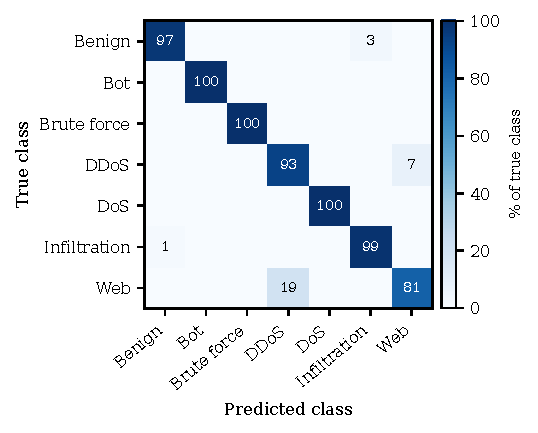
\includegraphics[width=0.92\columnwidth]{figures/fig_confusion_cic.pdf}
\caption{Row-normalised confusion matrix of FCHA on NF-CSE-CIC-IDS2018-v2, signature split, aggregated over 15 runs.}
\label{fig:confusion}
\end{figure}

\subsection{Unseen Attackers}
Table~\ref{tab:attacker} and Fig.~\ref{fig:attacker} report the leave-attacker-out split. It is far harder for every model: relative to the signature split, FCHA loses 21--23 points of balanced accuracy and the tree ensembles 10--27, and the variation across folds (SD 6--26 points) is larger than most differences between models.

On ToN-IoT-Network, FCHA has the highest mean (78.3\%), ahead of E-GraphSAGE-mean (74.5\%), Flow-MLP (74.0\%) and both tree ensembles (71.4\%, 71.9\%), and the lowest false-positive rate (6.0\% vs.\ 11.2--22.1\%). Its largest gain is fold F2, in which the dominant XSS attacker is unseen and only 537 XSS flows from other machines are available for training: FCHA reaches 90.6\% against 70.8\% for Flow-MLP and 66.0--67.7\% for the trees. Fold F3, whose only Backdoor attacker is held out with 143 Backdoor training flows from elsewhere, defeats every model (28.2--49.3\%). On NF-CSE-CIC-IDS2018-v2, FCHA (73.8\%) is level with the trees (73.3\%) and has the lowest false-positive rate (4.9\%, against 10.8\% for the random forest). On NF-ToN-IoT-v2, the centralised random forest is best (80.3\% vs.\ 71.4\%, $p=0.041$); FCHA's deficit comes almost entirely from fold F2, where Backdoor, Password and Scanning attackers are held out and its recall on those classes falls below 12\%.

Across the three datasets, no difference between FCHA and E-GraphSAGE-mean, Flow-MLP (except on NF-CSE-CIC-IDS2018-v2, $p=0.017$) or XGBoost is significant on this split. Host-mean is again significantly worse everywhere and collapses to 41.1\% with a 64.2\% false-positive rate on NF-ToN-IoT-v2.

\begin{table}[t]
\centering
\caption{Leave-attacker-out split (unseen attackers), IID clients. BA over supported classes. Mean $\pm$ SD over 15 runs; $p$ as in Table~\ref{tab:signature}.}
\label{tab:attacker}
\setlength{\tabcolsep}{2.6pt}
\footnotesize
\begin{tabular}{@{}lcccc@{}}
\toprule
Model & BA & F1 & FPR & $p$ \\
\midrule
\multicolumn{5}{@{}l}{\emph{NF-ToN-IoT-v2}}\\
FCHA (ours) & 71.4$\pm$14.1 & 72.5$\pm$16.0 & 11.8$\pm$9.3 & -- \\
E-GraphSAGE-mean & 72.7$\pm$13.1 & 73.9$\pm$14.3 & 19.1$\pm$17.7 & 0.757 \\
Host-mean & 41.1$\pm$7.3 & 39.7$\pm$8.4 & 64.2$\pm$15.7 & $<$0.001 \\
Flow-MLP & 73.4$\pm$14.3 & 70.9$\pm$17.6 & 16.3$\pm$14.5 & 0.757 \\
Random Forest$\dagger$ & \best{80.3}$\pm$6.2 & \best{77.8}$\pm$7.7 & \best{10.5}$\pm$12.1 & 0.041 \\
XGBoost$\dagger$ & 76.2$\pm$8.4 & 70.5$\pm$15.0 & 12.1$\pm$12.8 & 0.757 \\
\midrule
\multicolumn{5}{@{}l}{\emph{ToN-IoT-Network}}\\
FCHA (ours) & \best{78.3}$\pm$20.2 & \best{78.6}$\pm$19.5 & \best{6.0}$\pm$9.1 & -- \\
E-GraphSAGE-mean & 74.5$\pm$21.4 & 74.9$\pm$18.9 & 11.2$\pm$18.2 & 0.428 \\
Host-mean & 52.0$\pm$11.6 & 54.4$\pm$12.3 & 20.1$\pm$25.7 & $<$0.001 \\
Flow-MLP & 74.0$\pm$16.2 & 72.1$\pm$17.3 & 17.0$\pm$26.1 & 0.428 \\
Random Forest$\dagger$ & 71.4$\pm$19.0 & 71.1$\pm$17.1 & 16.5$\pm$25.5 & 0.428 \\
XGBoost$\dagger$ & 71.9$\pm$25.6 & 74.4$\pm$22.5 & 22.1$\pm$26.5 & 0.428 \\
\midrule
\multicolumn{5}{@{}l}{\emph{NF-CSE-CIC-IDS2018-v2}}\\
FCHA (ours) & \best{73.8}$\pm$8.5 & \best{71.1}$\pm$8.8 & \best{4.9}$\pm$2.4 & -- \\
E-GraphSAGE-mean & 70.5$\pm$8.8 & 66.5$\pm$13.0 & 5.0$\pm$3.0 & 0.321 \\
Host-mean & 57.2$\pm$10.9 & 52.3$\pm$15.1 & 6.4$\pm$4.4 & $<$0.001 \\
Flow-MLP & 68.8$\pm$7.5 & 63.3$\pm$11.8 & 13.8$\pm$6.2 & 0.017 \\
Random Forest$\dagger$ & 73.3$\pm$9.7 & 70.4$\pm$11.3 & 10.8$\pm$1.1 & 0.338 \\
XGBoost$\dagger$ & 73.3$\pm$9.4 & 65.5$\pm$17.7 & 6.3$\pm$1.8 & 0.762 \\
\bottomrule
\end{tabular}
\end{table}

\begin{figure*}[t]
\centering
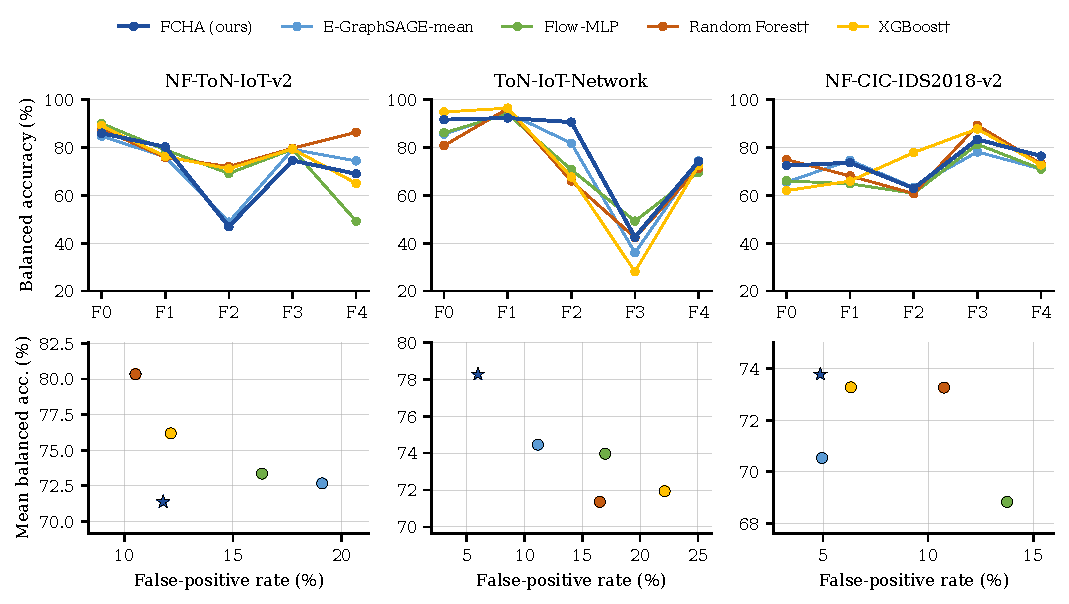
\includegraphics[width=\textwidth]{figures/fig_attacker.pdf}
\caption{Leave-attacker-out split. Top: balanced accuracy per fold (mean of 3 seeds); each fold holds out different attacker machines. Bottom: mean balanced accuracy against false-positive rate over all 15 runs; FCHA is marked with a star. Upper left is better.}
\label{fig:attacker}
\end{figure*}

\subsection{Cost of Federation and Ablations}
Table~\ref{tab:ablation} isolates the effect of federation and of the auxiliary loss. With IID clients, federated FCHA matches centralised FCHA within 0.3 points on all datasets (the 0.1-point gap on ToN-IoT-Network is significant but negligible). Dirichlet label skew costs 1.1, 0.1 and 2.0 points, more than it costs Flow-MLP on two of the datasets (0.5, 0.2, 0.5), but FCHA under skew still exceeds every flow-only model, including the centralised trees. The supervised contrastive term changes nothing measurable ($p\geq0.28$), so we do not include it in the final model.

\begin{table}[t]
\centering
\caption{Federation cost and ablations, signature split: balanced accuracy (\%), mean over 15 runs. All variants are federated over 5 clients except the centralised one ($\dagger$).}
\label{tab:ablation}
\setlength{\tabcolsep}{3.5pt}
\footnotesize
\begin{tabular}{@{}lccc@{}}
\toprule
Variant & NF-ToN-v2 & ToN-Net & NF-CIC-v2 \\
\midrule
FCHA, IID & 94.2 & 99.1 & 95.6 \\
FCHA, Dirichlet(0.5) & 93.1 & 99.0 & 93.6 \\
FCHA, centralised$\dagger$ & 94.5 & 99.2 & 95.6 \\
FCHA + SupCon, IID & 94.0 & 99.1 & 95.6 \\
\midrule
Flow-MLP, IID & 90.1 & 97.8 & 83.5 \\
Flow-MLP, Dirichlet(0.5) & 89.6 & 97.6 & 83.0 \\
\bottomrule
\end{tabular}
\end{table}

\subsection{What the Attention Attends To}
To test the mechanism directly we measure \emph{attention lift} on hosts whose flows span at least two classes. For query flows of class $c$ on such hosts, we divide the attention mass FCHA places on same-class neighbours by the fraction of same-class neighbours, i.e.\ the mass uniform averaging would assign; a lift above one means attention concentrates on similar traffic. Labels are used only for this post-hoc analysis. Table~\ref{tab:lift} shows that the lift is class-specific rather than uniform. On NF-CSE-CIC-IDS2018-v2 it is highest for web attacks (1.58), the class with the largest gain over mean aggregation (80.4\% vs.\ 72.8\% recall), and for Bot (1.37); on the two ToN-IoT datasets it is highest for DoS (1.89 and 1.66). On the leave-attacker-out split of NF-CSE-CIC-IDS2018-v2 it remains well above one for Bot (2.03), DDoS (1.56) and Brute force (1.42). For several majority classes the lift is near or below one, i.e.\ attention does not single out same-class traffic there, so the mechanism should be read per class and not as a general property.

\begin{table}[t]
\centering
\caption{Attention lift of FCHA on mixed-class hosts (signature split, mean over runs; $>$1: attention favours same-class flows).}
\label{tab:lift}
\setlength{\tabcolsep}{3.5pt}
\footnotesize
\begin{tabular}{@{}lclclc@{}}
\toprule
\multicolumn{2}{c}{NF-CIC-v2} & \multicolumn{2}{c}{NF-ToN-v2} & \multicolumn{2}{c}{ToN-Net} \\
\cmidrule(lr){1-2}\cmidrule(lr){3-4}\cmidrule(lr){5-6}
Web & \best{1.58} & DoS & \best{1.89} & DoS & \best{1.66} \\
Bot & 1.37 & DDoS & 1.28 & Password & 1.34 \\
DoS & 1.02 & Scanning & 1.18 & Scanning & 1.00 \\
Infiltration & 0.99 & Password & 1.08 & Benign & 0.91 \\
Benign & 0.97 & Benign & 0.90 & XSS & 0.94 \\
DDoS & 0.96 & XSS & 0.79 & DDoS & 0.75 \\
\bottomrule
\end{tabular}
\end{table}

\subsection{Communication and Sanity Checks}
Over a complete run (about 26--28 rounds with 5 clients), FCHA exchanges 199--205\,MB in total, compared with 143--146\,MB for E-GraphSAGE-mean and 80--86\,MB for Flow-MLP; per client and round this is 1.4\,MB. Only model weights are exchanged in volume: feature moments and confusion counts add a few kilobytes. Every shuffled-label run scored at chance (12.5\% balanced accuracy with 8 classes, 14.3\% with 7), confirming that no feature or preprocessing step leaks the label.

\section{Discussion}
\label{sec:discussion}

\emph{When does flow-conditioned context help?} The results separate two regimes. When an attack's traffic pattern or originating host has been seen in training, endpoint context is highly informative and the way it is aggregated matters: averaging alone is harmful when hosts mix classes (ToN-IoT) and adequate when they do not (CSE-CIC-IDS2018), while on this split flow-conditioned attention is never worse than mean aggregation and is clearly better on rare classes. When the attacker is new, endpoint context describes a host the model has never seen; it still helps FCHA where the held-out attack resembles traffic of other attackers (ToN-IoT-Network F2) and fails where an attack class has almost no training examples from other machines (F3) or where several classes are held out together (NF-ToN-IoT-v2 F2).

\emph{False alarms.} On two of three datasets FCHA attains its unseen-attacker accuracy with the lowest false-positive rate of all models: 6.0\% against 16.5--22.1\% for the tree ensembles on ToN-IoT-Network, and 4.9\% against 6.3--10.8\% on NF-CSE-CIC-IDS2018-v2. In operational settings, where analysts triage every alert, a detector with similar detection and fewer false alarms is preferable. On NF-ToN-IoT-v2 this advantage does not hold (11.8\% vs.\ 10.5\% for the random forest).

\emph{Evaluation practice.} Two observations generalise beyond our model. First, duplicate capping and signature grouping change conclusions: before capping, one of our test folds was two-thirds Bot traffic, and per-class results were unstable. Second, the drop of 10--27 points (21--23 for FCHA) between the signature and the leave-attacker-out splits shows that results on random or signature splits do not indicate how a detector will behave against new attacking machines. We recommend that federated NIDS papers report both.

\emph{Limitations.} (i) NF-ToN-IoT-v2 and ToN-IoT-Network come from the same testbed, so the study covers two independent networks; adding further testbeds would strengthen the generality of the conclusions. (ii) Clients are simulated partitions of one dataset; real deployments would have different hosts and traffic mixes per site. (iii) We use FedAvg without differential privacy or secure aggregation; the exchanged weights may leak information, and the accuracy cost of such mechanisms for FCHA remains to be measured. (iv) The test graph is built from a batch of test traffic; a streaming deployment would need windowed graphs, for which temporal graph models~\cite{rossi2020tgn} are a natural direction. (v) The tree ensembles are centralised references; federated tree learning would make the comparison fully symmetric.

\section{Conclusion}
We introduced FCHA, an edge classifier for federated IoT intrusion detection in which every flow attends to the flows of its endpoints with itself as the query, and evaluated it under a leakage-controlled protocol with duplicate capping, signature-grouped and leave-attacker-out splits, 15 runs per configuration and corrected significance tests. FCHA is the best (on one benchmark tied-best) model on unseen traffic patterns on all three benchmarks, improves rare-class recall by up to 52 points over flow-only models, and costs nothing relative to centralised training under IID clients. Host-level averaging, common in federated GNN detectors, loses up to 22 points. On unseen attackers, the hardest and most realistic setting, FCHA is competitive with centralised tree ensembles and produces markedly fewer false alarms on two of three datasets, but does not dominate. Closing this gap, for instance by letting the model learn when to trust host context, and adding formal privacy guarantees are the main directions for future work.

\section*{Data and Code Availability}
All configuration files, the code that produces every number and figure in this paper, and the per-run result records (one JSON line per run, including split audits and confusion matrices) are available at [repository URL].

\bibliographystyle{IEEEtran}
\begin{thebibliography}{99}

\bibitem{mcmahan2017fedavg}
H.~B. McMahan, E.~Moore, D.~Ramage, S.~Hampson, and B.~Ag{\"u}era~y~Arcas, ``Communication-efficient learning of deep networks from decentralized data,'' in \emph{Proc. 20th Int. Conf. Artificial Intelligence and Statistics (AISTATS)}, 2017, pp. 1273--1282.

\bibitem{li2020flchallenges}
T.~Li, A.~K. Sahu, A.~Talwalkar, and V.~Smith, ``Federated learning: Challenges, methods, and future directions,'' \emph{IEEE Signal Process. Mag.}, vol.~37, no.~3, pp. 50--60, 2020.

\bibitem{lo2022egraphsage}
W.~W. Lo, S.~Layeghy, M.~Sarhan, M.~Gallagher, and M.~Portmann, ``E-GraphSAGE: A graph neural network based intrusion detection system for IoT,'' in \emph{Proc. IEEE/IFIP Netw. Oper. Manage. Symp. (NOMS)}, 2022, doi: 10.1109/NOMS54207.2022.9789878.

\bibitem{chang2024eresgat}
L.~Chang and P.~Branco, ``Graph-based solutions with residuals for intrusion detection: The modified E-GraphSAGE and E-ResGAT algorithms,'' \emph{arXiv:2111.13597}, 2021.

\bibitem{altfaily2025fedgatsage}
F.~Al~Tfaily, Z.~Ghalmane, M.~A. Brahmia, H.~Hazimeh, A.~Jaber, and M.~Zghal, ``Graph-based federated learning approach for intrusion detection in IoT networks,'' \emph{Sci. Rep.}, vol.~15, art. 41264, 2025, doi: 10.1038/s41598-025-25175-1.

\bibitem{hamilton2017graphsage}
W.~L. Hamilton, R.~Ying, and J.~Leskovec, ``Inductive representation learning on large graphs,'' in \emph{Advances in Neural Information Processing Systems (NIPS)}, 2017.

\bibitem{arp2022dos}
D.~Arp, E.~Quiring, F.~Pendlebury, A.~Warnecke, F.~Pierazzi, C.~Wressnegger, L.~Cavallaro, and K.~Rieck, ``Dos and don'ts of machine learning in computer security,'' in \emph{Proc. 31st USENIX Security Symp.}, 2022, pp. 3971--3988.

\bibitem{velickovic2018gat}
P.~Veli{\v{c}}kovi{\'c}, G.~Cucurull, A.~Casanova, A.~Romero, P.~Li{\`o}, and Y.~Bengio, ``Graph attention networks,'' in \emph{Proc. Int. Conf. Learning Representations (ICLR)}, 2018.

\bibitem{ngo2025attribute}
T.~Ngo, J.~Yin, Y.-F. Ge, and H.~Wang, ``Optimizing IoT intrusion detection---A graph neural network approach with attribute-based graph construction,'' \emph{Information}, vol.~16, art. 499, 2025, doi: 10.3390/info16060499.

\bibitem{rossi2020tgn}
E.~Rossi, B.~Chamberlain, F.~Frasca, D.~Eynard, F.~Monti, and M.~Bronstein, ``Temporal graph networks for deep learning on dynamic graphs,'' \emph{arXiv:2006.10637}, 2020.

\bibitem{zhao2018noniid}
Y.~Zhao, M.~Li, L.~Lai, N.~Suda, D.~Civin, and V.~Chandra, ``Federated learning with non-IID data,'' \emph{arXiv:1806.00582}, 2018.

\bibitem{hsu2019noniid}
T.-M.~H. Hsu, H.~Qi, and M.~Brown, ``Measuring the effects of non-identical data distribution for federated visual classification,'' \emph{arXiv:1909.06335}, 2019.

\bibitem{liu2024fedgnn}
R.~Liu, P.~Xing, Z.~Deng, A.~Li, C.~Guan, and H.~Yu, ``Federated graph neural networks: Overview, techniques, and challenges,'' \emph{arXiv:2202.07256}, 2022.

\bibitem{wang2025fedstgcn}
Y.~Wang, J.~Li, Z.~Han, P.~Cheng, and R.~Kumar, ``FedSTGCN: A novel federated spatiotemporal graph learning-based network intrusion detection method for the Internet of Things,'' \emph{Front. Inf. Technol. Electron. Eng.}, vol.~26, no.~7, pp. 1164--1179, 2025.

\bibitem{youm2025sampling}
S.~Youm and T.~Kim, ``Enhancing federated intrusion detection with class-specific dynamic sampling,'' \emph{Appl. Sci.}, vol.~15, art. 5067, 2025, doi: 10.3390/app15095067.

\bibitem{sarhan2021netflow}
M.~Sarhan, S.~Layeghy, N.~Moustafa, and M.~Portmann, ``NetFlow datasets for machine learning-based network intrusion detection systems,'' \emph{arXiv:2011.09144}, 2020.

\bibitem{sarhan2022standard}
M.~Sarhan, S.~Layeghy, and M.~Portmann, ``Towards a standard feature set for network intrusion detection system datasets,'' \emph{Mobile Netw. Appl.}, vol.~27, no.~1, pp. 357--370, 2022, doi: 10.1007/s11036-021-01843-0.

\bibitem{moustafa2021toniot}
N.~Moustafa, ``A new distributed architecture for evaluating AI-based security systems at the edge: Network TON\_IoT datasets,'' \emph{Sustain. Cities Soc.}, vol.~72, art. 102994, 2021.

\bibitem{alsaedi2020toniot}
A.~Alsaedi, N.~Moustafa, Z.~Tari, A.~Mahmood, and A.~Anwar, ``TON\_IoT telemetry dataset: A new generation dataset of IoT and IIoT for data-driven intrusion detection systems,'' \emph{IEEE Access}, vol.~8, pp. 165130--165150, 2020, doi: 10.1109/ACCESS.2020.3022862.

\bibitem{sharafaldin2018cicids}
I.~Sharafaldin, A.~H. Lashkari, and A.~A. Ghorbani, ``Toward generating a new intrusion detection dataset and intrusion traffic characterization,'' in \emph{Proc. 4th Int. Conf. Inf. Syst. Security Privacy (ICISSP)}, 2018, pp. 108--116.

\bibitem{breiman2001rf}
L.~Breiman, ``Random forests,'' \emph{Mach. Learn.}, vol.~45, pp. 5--32, 2001.

\bibitem{chen2016xgboost}
T.~Chen and C.~Guestrin, ``XGBoost: A scalable tree boosting system,'' in \emph{Proc. 22nd ACM SIGKDD Int. Conf. Knowl. Discov. Data Min.}, 2016, pp. 785--794.

\bibitem{vaswani2017attention}
A.~Vaswani, N.~Shazeer, N.~Parmar, J.~Uszkoreit, L.~Jones, A.~N. Gomez, {\L}.~Kaiser, and I.~Polosukhin, ``Attention is all you need,'' in \emph{Advances in Neural Information Processing Systems 30}, 2017, pp. 5998--6008.

\bibitem{johnson2019imbalance}
J.~M. Johnson and T.~M. Khoshgoftaar, ``Survey on deep learning with class imbalance,'' \emph{J. Big Data}, vol.~6, art. 27, 2019, doi: 10.1186/s40537-019-0192-5.

\bibitem{cui2019classbalanced}
Y.~Cui, M.~Jia, T.-Y. Lin, Y.~Song, and S.~Belongie, ``Class-balanced loss based on effective number of samples,'' in \emph{Proc. IEEE/CVF Conf. Comput. Vis. Pattern Recognit. (CVPR)}, 2019, pp. 9268--9277.

\bibitem{khosla2020supcon}
P.~Khosla, P.~Teterwak, C.~Wang, A.~Sarna, Y.~Tian, P.~Isola, A.~Maschinot, C.~Liu, and D.~Krishnan, ``Supervised contrastive learning,'' in \emph{Advances in Neural Information Processing Systems (NeurIPS)}, 2020.

\bibitem{wilcoxon1945}
F.~Wilcoxon, ``Individual comparisons by ranking methods,'' \emph{Biometrics Bull.}, vol.~1, no.~6, pp. 80--83, 1945.

\bibitem{holm1979}
S.~Holm, ``A simple sequentially rejective multiple test procedure,'' \emph{Scand. J. Statist.}, vol.~6, no.~2, pp. 65--70, 1979.

\end{thebibliography}

\end{document}
